\begin{figure}
	\centering
	\setlength{\imagewidth}{100mm}%
	\setlength{\imageheight}{\imagewidth}%
	\newdimen\radiuscycle
	\radiuscycle=0.08\imagewidth
	%
	\DTLsetseparator{,}%
	\DTLloaddb[noheader,keys={x,y}]{dbvertex}{figures/data/pseudo_EdS_sommet/xy_vertex.dat}%
	\DTLloaddb[noheader,keys={x,y}]{dbfacelabel}{figures/data/pseudo_EdS_sommet/xy_facelabel.dat}%
	\DTLloaddb[noheader,keys={x,y}]{dbedgelabel}{figures/data/pseudo_EdS_sommet/xy_edgelabel.dat}%
	\begin{tikzpicture}[
		x=\imagewidth,
		y=\imageheight
	]
		%
		\node[anchor=south west, inner sep=0] at (0,0) {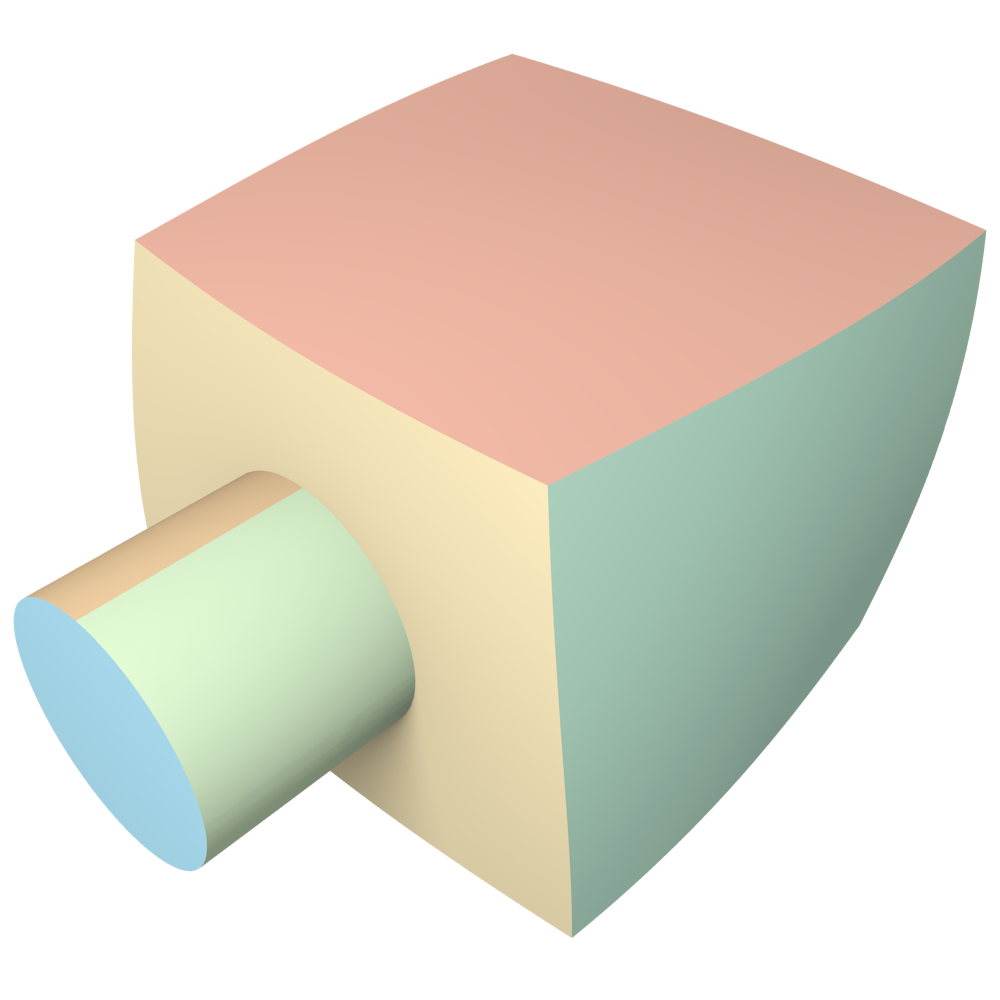
\includegraphics[width=\imagewidth]{pseudo_EdS_sommet/aretes_faces_incidentes}};
		%
		\DTLassign{dbvertex}{1}{\vx=x, \vy=y}%
		\coordinate (v) at (\vx, \vy);
		\fill[black] (v) circle (1.3pt);
		\draw[->] (v) + (-60:\radiuscycle) arc (-60:240:\radiuscycle);
		%
		{\transparent{0.55}%
			\DTLforeach{dbfacelabel}{\flx=x, \fly=y}%
			{%
				\node at (\flx, \fly) {$\brepface_{\arabic{DTLrowi}}$};
			}%
		}
		%
		\DTLforeach{dbedgelabel}{\elx=x, \ely=y}%
		{%
			\node at (\elx, \ely) {$\brepedge_{\arabic{DTLrowi}}$};
			\draw[line width=0.7pt, line cap=round, shorten >= 0.35pt] 
				plot file {figures/data/pseudo_EdS_sommet/xy_edge_\arabic{DTLrowi}.dat};
		}%
		%
		\node[above] at (v) {$\brepvertex$};
	\end{tikzpicture}
	\DTLgdeletedb{dbvertex}%
	\DTLgdeletedb{dbfacelabel}%
	\DTLgdeletedb{dbedgelabel}%
	\caption{Cycle des arêtes et faces incidentes à un sommet du modèle \brep.}
	\label{fig:cycle_aretes_faces_incidentes}
\end{figure}